% article example for classicthesis.sty
\documentclass[10pt,a4paper]{article} % KOMA-Script article scrartcl
\usepackage{import}
\usepackage{xifthen}
\usepackage{pdfpages}
\usepackage{transparent}
\newcommand{\incfig}[1]{%
    \def\svgwidth{\columnwidth}
    \import{./figures/}{#1.pdf_tex}
}
\usepackage{lipsum}     %lorem ipsum text
\usepackage{titlesec}   %Section settings
\usepackage{titling}    %Title settings
\usepackage[margin=10em]{geometry}  %Adjusting margins
\usepackage{setspace}
\usepackage{listings}
\usepackage{amsmath}    %Display equations options
\usepackage{amssymb}    %More symbols
\usepackage{xcolor}     %Color settings
\usepackage{pagecolor}
\usepackage{mdframed}
\usepackage[spanish]{babel}
\usepackage[utf8]{inputenc}
\usepackage{longtable}
\usepackage{multicol}
\usepackage{graphicx}
\graphicspath{ {./Images/} }
\setlength{\columnsep}{1cm}

% ====| color de la pagina y del fondo |==== %
\pagecolor{black}
\color{white}



\begin{document}
    %========================{TITLE}====================%
    \title{{  5th laboratory  }}
    \author{{Rodrigo Castillo}}
    \date{\today}

    \maketitle


     % ====| Loguito |==== %
    
\includegraphics[width=0.1\linewidth]{negro_cara.png}
    %=======================NOTES GOES HERE===================%

    \section{Read the introduction to "A Crash Course In X86 Disassembly" and
    identify 3 reasons to do disassembly over a malware:}

        \begin{enumerate}
            \item {Dissasembly can be used to understand the malware without
                running it}
            \item {Disassembly is usefull for reconstruct the code of a
                malware, sometimes there are processes that cannot be seen on
                process monitor, thats why looking at the assembly code can be
                usefull}
            \item {it also works for understand how malware works, personally,
                i use it for hacking on binary exploitation contests}
        \end{enumerate}

    \section{Read the section "Levels of abstraction" and explain the
        difference between high-level language, low-level language and machine
        code.}

        \color{red} low level programming ... \color{white}
        \begin{itemize}
            \item {the code is readed by a compiler that transforms code into
                machine code}
            \item {its supposed to be more portable}
            \item {the number and abstractions for instructions is lower, you
                need more instructions to tell the machine to do the same than
                an high level programming language}
            \item {instructions runs faster than in a high level programming
                language because compiler dont need to assume machine
                instructions}
            \item {machine code can be disassembly}
        \end{itemize}

        \color{red} high level programming language ... \color{white}
        \begin{itemize}
            \item {the code is readed by a interoreter line by line}
            \item {its supposed to be less portable but i think is more
                portable nowdays}
            \item {coding is faster because interpreter assumes a lot of
                machine code instructions}
            \item {instructions runs slower, but, for example, python
                interpreter transforms heavy algorithms into low level
            programming porgrams for make it faster}
            \item {its not necesary to disassembly because investigator can
                read the code of the program, sometimes is encoded but thats
                another prolem that occurs also with low level programming
                languages}
        \end{itemize}
        there are a lot of differences between low level and high level
        programming languages but listing all of them is impossible in this
        section

    \section{Python may be considered a hardware, microcode, machine code,
    low-level language, high-level language or interpreted language? Why?}
        Pythons is a high level language

    \section{What is the difference between an application written in C++ and
    the equivalent application written in Python?}
        \begin{itemize}
            \item {application in c++ is faster but the code is also larger}
            \item {application in c++ is compiled and in python is interpreted}
            \item {application in c++ its supposed to be more portable}
        \end{itemize}

    \section{Why the assembly dialect must not be the same for all the PC
        architectures? Why is useful to study x86 dialect?}

        Assembly language is machine code, that means that it can run or not
        depends on the machine , there are several architectures for computers,
        x64 , x86 , ARM , 8 bit ... $ etc  $  , that means that instructions
        for an architecture not necesary will run in other architectures,
        however, the most used architecture nowdays is $ x64  $  and codes
        compiled for $ x86  $ runs in $ x86  $ machines and in $ x64  $
        machines, that mean that if an attacker want to make malware, the best
        option for him is making it for $ x86  $ because most of the machines
        in the world will run it .

    \section{Read the section "The x86 architecture" and explain the utility of
    "registers"}
        registers are the same as variables in the code, they store hex numbers
        inside them and use it for writing in other spaces or other registers

    \section{Read the section "Main Memory" and explain the differences between
    Stack, Heap, code and Data.}
        \begin{itemize}
            \item {in $ data  $ its stored all the static variables that are not going to be modified}
            \item {in $ code  $  instructions are loaded}
            \item {in $ heap  $  all dinamyc variables are loaded, all the
                variables that are modified constantly.}
            \item {in $ stack  $  all local variables , function declarations,
                memory spaces are loaded}
        \end{itemize}

    \section{Read the section "Instructions" and explain what are opcodes
    (operation codes)}
        assembly have several different instructions , opcodes are instructions
        in assembly between registers, such as mv , jmp , jeq , jne , sub , add , push ...
        \\
        are instructions that lead the machine to perform compiled code
        instructions , for example, jmp instruction overwrite $ eip  $  to an
        instruction, or $ add  $ add a hex value over a register $ push  $ loads a hex into a space of memory, all the
        several instructions are derivates and combinations from those instructions.

    \section{What is the difference between little-endian and big-endian format?}
        imagine that we are going to encode the number $ 0xcafebabe  $ ...
        \begin{itemize}
            \item {in big endian would be xca xfe xba xbe}
            \item {in little endian would be  xbe xba xfe xca }
        \end{itemize}

    \section{Put an example of 3 types of instructions used in x86
        architectures and explain its purpose (mov, add, push, call, xor, cmp).
        Full documentation:
        https://software.intel.com/content/www/us/en/develop/download/intel-64-and-ia-32-architectures-sdm-combined-volumes-1-2a-2b-2c-2d-3a-3b-3c-3d-and-4.html
        Pag 116.}
        i already made it in a previus section

    \section{Explain the difference between Immediate, Register and Memory
    Address? Give an example of each one.}
        inmediate is when an instruction runs without searching for a value in
        a register , for example push 0xf that runs this instruction into the
        stack, register and memory would be for example mov eax 0xf

    \section{How many registers exists in a X86 architecture and what are used
    for? (General, Segment, Status, Instruction Pointer)}
        there are 8 registers of 16 bits,  8 of 32 bits , there is the flag
        register and most important one is $ eip  $ that is instruction pointer
        that store the next instruction , ones of them are used for storing hex
        values into memory spaces and others are used for storing hex value
        into other registers

    \section{What is the purpose of NOP instruction?}
        its no operation instruction , it stands for when the programmer want
        to freeze a register

    \section{What is the difference between move and lea (load effective
    address) instructions}

        as i understand, mov moves a value from a register to another ,
        lea safe the value into the register


    \section{  Find the address and PE Section where the imported function gethost-byname resides }
        i found service main at 0x1000cf30  and gethost-byname in 0x1000d02e
        \\
        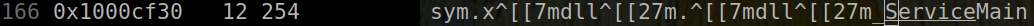
\includegraphics[width=0.8\linewidth]{service.png}
        \\



















































    %=======================NOTES ENDS HERE===================%

    % bib stuff
    \nocite{*}
    \addtocontents{toc}{{}}
    \addcontentsline{toc}{section}{\refname}
    \bibliographystyle{plain}
    \bibliography{../Bibliography}
\end{document}
